\section{Computational aspects}
\label{Sec1:computationalAspects}
Several computational issues arise when implementing the exact solution (which has been implemented in \href{mathworks.com}{\MATLAB}). The source code can be downloaded from GitHub at \href{https://github.com/Zetison/e3Dss}{https://github.com/Zetison/e3Dss}. In this section, a discussion of some of these issues will be presented.

\subsection{Matrix manipulations}
Note that the only complex valued matrix entries of $\vec{H}_n$ are the first two entries in the first column. So instead of using a complex matrix solution routine to solve the system, one can exploit this fact to solving a real valued linear system of equations with two right hand sides. Refer to Fender~\cite[pp. 18-20]{Fender1972sfa} for details. Moreover, Fender shows that some further matrix manipulation may reduce the overall computational time by 30\% (when doing a frequency sweep). By using the same ideas, the size of $\vec{H}_n$ can be reduced from $6M$ to $4M$.

Note that for $n>0$, column number $2l$, $l=1, 2, \dots, 3M$, of $\vec{H}_n$ contains entries which are linear combinations of $\besselj_n$ and $\besselj_{n+1}$ (and no spherical Bessel functions of second kind), while column number $2l-1$, $l=1, 2, \dots, 3M$, of $\vec{H}_n$ contains entries which are linear combinations of $\bessely_n$ and $\bessely_{n+1}$. So since
\begin{equation}
	\lim_{n\to\infty} |\besselj_n(\zeta)| = 0\quad\text{and}\quad \lim_{n\to\infty} |\bessely_n(\zeta)| = \infty,
\end{equation}
(which is illustrated in \Cref{Fig1:besselPlotLargeN})
\begin{figure}
	\centering
	\begin{subfigure}[t]{0.48\textwidth}
		\centering
		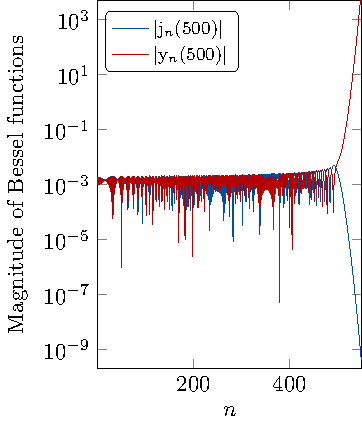
\includegraphics{besselPlotLargeN_1}
		\caption{Magnitude of Besselfunctions ploted for ${n\in[0,550]}$.}
	\end{subfigure}
	~
	\begin{subfigure}[t]{0.48\textwidth}
		\centering
		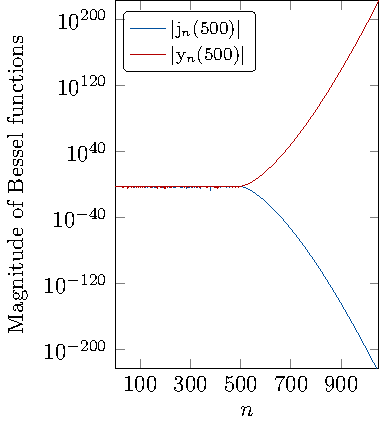
\includegraphics{besselPlotLargeN_2}
		\caption{Magnitude of Besselfunctions ploted for $n\in[0,1050]$.}
	\end{subfigure}
	\caption{Illustration of the asymptotic behavior, of the spherical Bessel functions of first ($\besselj_n(x)$) and second ($\bessely_n(x)$) kind, as a function of $n$, for a fixed argument $x=500$.}
	\label{Fig1:besselPlotLargeN}
\end{figure}
the matrix $\vec{H}_n$ becomes poorly scaled for large $n$. This issue can be solved by scaling the matrix with a (diagonal) preconditioning matrix $\vec{P}_n$ where the diagonal entries are given by the maximal modulus of the corresponding column vectors of $\vec{H}_n$. Defining the vector $\tilde{\vec{C}}_n = \vec{P}_n\vec{C}_n$ and solving the system $\tilde{\vec{H}}_n\tilde{\vec{C}}_n = \vec{D}_n$ with $\tilde{\vec{H}}_n = \vec{H}_n \vec{P}_n^{-1}$, the solution is obtained by $\vec{C}_n = \vec{P}_n^{-1}\tilde{\vec{C}}_n$. In \Cref{Fig1:Spy2K,Fig1:Spy2K2} the magnitude of the entries in $\vec{H}_n$ is visualized before and after preconditioning, respectively.
\begin{figure}
	\centering
	\begin{subfigure}{\textwidth}
		\centering
		\includegraphics[scale=1]{spy_K_1}
		\caption{Before preconditioning.}
		\label{Fig1:Spy2K}
	\end{subfigure}
	\par\bigskip
	\begin{subfigure}{\textwidth}
		\centering
		\includegraphics{spy_K_2}
		\caption{After preconditioning.}
		\label{Fig1:Spy2K2}
	\end{subfigure}
	\caption{\textbf{Matrix manipulations}: Plot of the magnitude of the matrix entries of $\vec{H}_{300}$ and $\tilde{\vec{H}}_{300}$.}
	\label{Fig1:SpyK}
\end{figure}
This example is the matrix $\vec{H}_{300}$ of the S135 benchmark problem (described in \Cref{Subsec1:benchmarkProblem}) at $f=\SI{30}{kHz}$. The condition number was improved from $\operatorname{cond}(\vec{H}_{300}) \approx 7.4\cdot 10^{278}$ to $\operatorname{cond}(\tilde{\vec{H}}_{300}) \approx 9.4\cdot 10^4$.

\subsection{Series evaluation}
\label{Subsec1:seriesEval}
As the series involves summation over infinitely many terms, the series needs to be truncated at some number $n=N_\varepsilon$. Denote by $p_1^{(N)}$, the truncated sum for the scattered pressure in the outer domain (\Cref{Eq1:Summary_pm}), 
\begin{align}\label{Eq1:truncated_p1}
p_1^{(N)}(r,\vartheta) &= \sum_{n=0}^N Q_n^{(0)}(\vartheta) C_{1,n}^{(1)} \hankel^{(1)}_n(k_1 r),
\end{align}
and correspondingly for the other fields in \Cref{Eq1:Summary_pm,Eq1:Summary_pM1,Eq1:Summary_u}.
In~\cite[pp. 32-35]{Ihlenburg1998fea}, Ihlenburg discusses such a value based on the decay of Bessel functions, in which he suggests using $N\approx 2kr$. In this work, however, the summation is terminated whenever the magnitude of term $n=N_\varepsilon$ divided by the magnitude of the partial sum (based on the first $N_\varepsilon+1$ terms) is less than some prescribed tolerance $\varepsilon$. Typically machine epsilon is used for this number, i.e. $\varepsilon \approx 2.220446\cdot 10^{-16}$. As with the suggestion of Ihlenburg, the number of terms, $N_\varepsilon$, grows linearly with the frequency. The computational complexity of the problem is thus $\bigoh(\omega)$. 

The solution is often needed at several points, or frequencies (or a combination of both). In this case, one should compute the solutions at all points at once, such that the calls to the implemented Bessel functions are minimized.

\subsection{Round-off errors}
\label{Subsec1:RoundoffErrors}
Although the products $A_{m,n}^{(2)}S_{j,n}^{(2)}(\zeta)$, $B_{m,n}^{(2)}T_{j,n}^{(2)}(\zeta)$ and $C_{m,n}^{(2)}Z_n^{(2)}(\eta)$ all goes to zero as $n\to\infty$, the functions $S_{j,n}^{(2)}(a_m r)$, $T_{j,n}^{(2)}(\zeta)$ and $Z_n^{(2)}(\eta)$ does not. In fact, these functions become unbounded when $n\to\infty$ because they are all superposition of Bessel functions of second kind with this property. So, since the floating point number has an upper bound\footnote{For double precision this is typically $V_{\mathrm{max}} \approx 1.797693134862316\cdot 10^{308}$.}, there is a limit to the number of terms that can be used. 

A naive solution to this problem is to try higher precision, which can easily be done with MATLAB symbolic class. This, however, increases the computational time drastically. 

In \Cref{Fig1:errorsS123_ASI-6NN} several round-off phenomena which typically arises are illustrated.
\begin{figure}
	\centering
	\begin{subfigure}[t]{0.49\textwidth}
		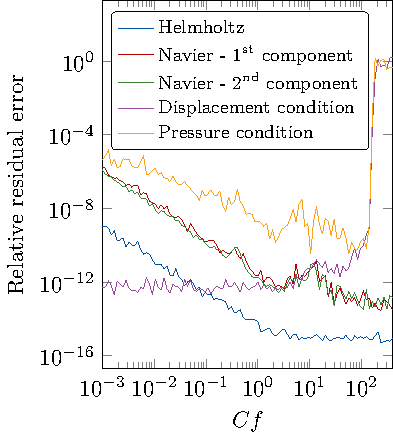
\includegraphics[width=\textwidth]{errors_S135_SSBC_1}
		\caption{Double precision, $\varepsilon \approx 10^{-16}$}
	\end{subfigure}%
	\hspace*{0.02\textwidth}%
	\begin{subfigure}[t]{0.49\textwidth}
		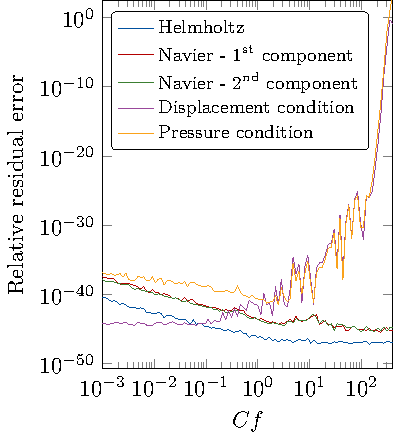
\includegraphics[width=\textwidth]{errors_S135_SSBC_2}
		\caption{Symbolic precision $\varepsilon \approx 10^{-40}$}
	\end{subfigure}
	\caption{\textbf{Round-off errors}: Residual errors for the governing equations and boundary conditions. The use of symbolic precision in MATLAB illustrate that the errors are due to round-off errors. The relative residual formulas for the Helmholtz equation, the first and second components of the Navier equation, the displacement condition and the pressure conditions are given by \Cref{Eq1:residualHelmhotlz,Eq1:residualNavier1,Eq1:residualNavier2,Eq1:residualDisplacement,Eq1:residualPressure}, respectively.}
	\label{Fig1:errorsS123_ASI-6NN}
\end{figure}
The specific example used here is the S135 benchmark problem with SSBC (described in \Cref{Subsec1:benchmarkProblem}). The incident wave, $p_{\mathrm{inc}}$, is a plane wave traveling in the direction given by $\vartheta=\ang{60}$ and $\varphi=\ang{240}$ (see \Cref{Sec1:resultsDisc}). An uniform (relative to the spherical coordinate system) set of sample points are distributed in all domains\footnote{It is placed 32 points in each domain except for the inner domain with 25 points. The distribution of point in the radial direction in the exterior domain is limited to the interval $[R_{0,1}, 2R_{0,1}]$.} where the residual error in the Helmholtz equation (\Cref{Eq1:helmholtz}), the $1^{\mathrm{st}}$ and $2^{\mathrm{nd}}$ component of Navier's equation in spherical coordinates (\Cref{Eq1:navierSphericalSimplified1,Eq1:navierSphericalSimplified2}, respectively), the displacement condition (\Cref{Eq1:firstBC}) and the pressure condition (\Cref{Eq1:secondBC}), is measured. By using the infinity norm, $\|\cdot\|_\infty$, for each residual, and dividing by the magnitude of the terms involved, the relative residual error is obtained. The maximal relative residual in all domains can then be calculated. In particular, these relative residual errors are given by
\begin{align}%
	&\max_{1\leq m\leq M+1}\frac{\left\|\left(\nabla^2 + k_m^2\right)p_m\right\|_\infty}{\left\|k_m^2p_m\right\|_\infty}\label{Eq1:residualHelmhotlz}\\
	&\resizebox{0.9\textwidth}{!}{$\displaystyle\max_{1\leq m\leq M}\frac{\left\|\pderiv{\sigma_{\mathrm{rr},m}}{r} + \frac{1}{r}\pderiv{\sigma_{\mathrm{r}\upvartheta,m}}{\vartheta} + \frac{1}{r}\left(2\sigma_{\mathrm{r}\mathrm{r},m} - \sigma_{\upvartheta\upvartheta,m} - \sigma_{\upvarphi\upvarphi,m} + \sigma_{\mathrm{r}\upvartheta,m}\cot\vartheta\right) + \omega^2\rho_{\mathrm{s},m}u_{\mathrm{r},m}\right\|_\infty}{\left\|\omega^2\rho_{\mathrm{s},m}u_{\mathrm{r},m}\right\|_\infty}$}\label{Eq1:residualNavier1}\\
	&\resizebox{0.9\textwidth}{!}{$\displaystyle\max_{1\leq m\leq M}\frac{\left\|\pderiv{\sigma_{\mathrm{r}\upvartheta,m}}{r} + \frac{1}{r}\pderiv{\sigma_{\upvartheta\upvartheta,m}}{\vartheta} + \frac{1}{r}\left[(\sigma_{\upvartheta\upvartheta,m} - \sigma_{\upvarphi\upvarphi,m})\cot\vartheta + 3\sigma_{\mathrm{r}\upvartheta,m} \right] +\omega^2\rho_{\mathrm{s},m}u_{\upvartheta,m}\right\|_\infty}{\left\|\omega^2\rho_{\mathrm{s},m}u_{\upvartheta,m}\right\|_\infty}\label{Eq1:residualNavier2}$}\\
	&\max_{1\leq m\leq M}\frac{\left\|\rho_{\mathrm{f}} \omega^2 u_{\mathrm{r}} - \pderiv{p_{\mathrm{tot}}}{r}\right\|_\infty}{\left\|\pderiv{p_{\mathrm{tot}}}{r}\right\|_\infty}\label{Eq1:residualDisplacement}\\
	&\max_{1\leq m\leq M}\frac{\left\|\sigma_{\mathrm{rr}} + p_{\mathrm{tot}}\right\|_\infty}{\left\|p_{\mathrm{tot}}\right\|_\infty}.\label{Eq1:residualPressure}%$}
\end{align}
By comparing these error results for both double precision and symbolic precision in MATLAB, one can conclude that the errors indeed originate from round-off errors. When using double precision, the summation is ended whenever $|\bessely_n(\eta)| > 10^{290}$, such that invalid solutions is obtained for sufficiently large $n$. Since one needs to have enough terms for the solution to converge, and at the same time have to avoid computing $\bessely_n(\eta)$ for low $\eta$ (and large $n$), the following bound on the frequency based on experimental data is suggested
\begin{equation}\label{Eq1:Upsilon}
	f \lesssim \frac{100}{C},\qquad C =\left(\frac{R_{0,1}}{c_{\mathrm{f},1}}\right)^{\frac{3}{2}}\frac{1}{\sqrt{\Upsilon}}
\end{equation}
with
\begin{equation*}
	\Upsilon = \min\left\{\min_{1\leq m\leq M}\frac{R_{1,m}}{\max\{c_{\mathrm{s,1},m},c_{\mathrm{s,2},m}\}},\min_{1\leq m\leq M}\frac{R_{0,m}}{c_{\mathrm{f},m}}\right\}
\end{equation*}
where $c_{\mathrm{s,1},M}$ and $c_{\mathrm{s,2},M}$ is the transverse and longitudinal wave velocity for the $M^{\mathrm{th}}$ spherical shell, respectively. The constant $\Upsilon$ corresponds to the lowest argument $\eta$ used for the Bessel functions of second kind. An addendum will be given to yield more numerical evidence for this bound. In particular, plots similar to the ones in \Cref{Fig1:errorsS123_ASI-6NN} will be presented for all benchmarks and corresponding boundary conditions in \Cref{Subsec1:benchmarkProblem}. However, it would certainly be possible to construct models in which this bound is not valid.

One can also observe significant round-off errors for very low frequencies which is again due to the evaluation of the spherical Bessel functions of the second kind with the property
\begin{equation}
	\lim_{\zeta\to 0} |\bessely_n(\zeta)| = \infty.
\end{equation}
Finally, observe that problems for higher frequencies also occur when using the symbolic class in MATLAB (even though the summation is not terminated prematurely), which calls for a more mathematically sound way of solving this issue. To avoid evaluating the Bessel functions directly, one could include a scaling such that one need to evaluate products of the form $\besselj_n(\xi)\bessely_n(\eta)$, $\besselj_{n+1}(\xi)\bessely_n(\eta)$, $\besselj_n(\xi)\bessely_{n+1}(\eta)$ and $\besselj_{n+1}(\xi)\bessely_{n+1}(\eta)$ (which will be $0\cdot\infty$ type products). One would then probably need to use relations like~\cite[\href{http://functions.wolfram.com/03.21.26.0047.01}{03.21.26.0047.01} and \href{http://functions.wolfram.com/03.21.26.0049.01}{03.21.26.0049.01}]{WolframResearch2016m}
\begin{align}
\besselj_n(\sqrt{z})\bessely_n(\sqrt{z}) &=-\frac{\sqrt{\PI}}{2}G_{1,3}^{2,0}\left(z\Bigg\vert\begin{matrix}
	0\\
	-\frac{1}{2}, n, -n-1
	\end{matrix}\right)\\
	\besselj_{n+1}(\sqrt{z})\bessely_n(\sqrt{z}) &=\frac{\sqrt{\PI}}{2}G_{2,4}^{2,1}\left(z\Bigg\vert\begin{matrix}
	0,-\frac{1}{2}\\
	0, n+\frac{1}{2},-1,-n-\frac{3}{2}
	\end{matrix}\right)
\end{align}
where $G$ is the Meijer G-function. This investigation is left as future work.





